\documentclass[12pt,twocolumn,twoside]{conference}   %%
\usepackage[german, english]{babel}                  %%
%%% Vorgaben %%%%%%%%%%%%%%%%%%%%%%%%%%%%%%%%%%%%%%%%%%


\title{Technique and procedures of business analytics}
 
\author{Sean Payne}

\begin{document}
\twocolumn[
  \begin{@twocolumnfalse}
  \maketitle\thispagestyle{firststyle}
    \begin{abstract}
    \vspace{8pt}
    
The aim of this paper is to provide an overview of the importance of business analytics. Furthermore, different approaches and typical application techniques of the business analytics models are discussed. Subsequently, the procedure of the so-called Knowledge Discovery in Databases (KDD) will be discussed and there especially the Data Mining. Finally, predictive analytics and the methodological and architectural approaches to be recommended are presented.

    \end{abstract}
    \vspace{16pt}
  \end{@twocolumnfalse}
]
\section{Introduction}
In the past, it was the job of a so-called controller to check and juggle the economic figures of a company to gather information about its economic efficiency. But nowadays this has changed. The task area of a controller has become much more technically adept and complex in the last decades. Nowadays, one of the main tasks of a controller is to apply so-called "business analytics" in order to keep the company economically, so that it can still be represented on the market. But what exactly are these business analytics? In order to provide a better insight into business analytics, this paper is dealing with answering the following questions.

\begin{enumerate}
\item What exactly are business analytics?
\item What is the general procedure in business analytics?
\item Why would you use business analytics?
\item Why is so much attention paid to business analytics?
\item Fields of application of business analytics
\item What has to be considered with business analytics?
\item What kind of business analytics tools are available?
\end{enumerate}


In the course of business analytics, there are many methods and tools to analyse and later evaluate large amounts of data. It is not a big problem to evaluate data which only change in individual values. But what if the received data consists of an uneven structure? For the mentioned case of the so-called "heterogeneous data" is it usual to use the method of Knowledge Discovery in Databases (KDD), which is often confused with Data Mining. This is also a topic, where this Paper is heading to.

Another tool of the controller is the so called predictive analytics. Predictive analytics describes a process that uses and evaluates historical data to predict future events. In contrast to knowledge discovery in databases, predictive analytics is not only about evaluating the data and using this evaluation to initiate the next steps, but rather about generating models for that evaluation (cf. Baars \cite{1}). 




\section{Business Analytics}
\subsection{What are business analytics?}
Business analytics is described as a process of researching and evaluating historical data, which provides information about a possible future orientation for the company. As already described above, they are mainly seen as a kind of tool of the controller. With the help of business analytics, historical data of the company or the data of the company environment are used to make decisions as to what course the company should take in order, to be able to operate economically in the future. It is important to understand that business analytics is an ongoing process that is divided into several phases, which are going to be described in the following subareas.

\subsection{Business Analytics - General procedure}
\begin{figure}[H]
\centering
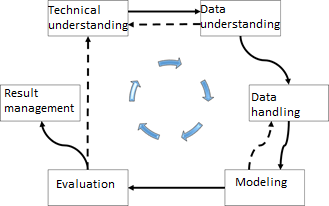
\includegraphics[width=8cm]{Abbildungen/Business_Analytics_Process.png}
\caption{Business Analytics Process \cite{10}}\label{visina8}
\end{figure}

As you can see in Figure 1, has business analytics to be seen as an ongoing process. This ongoing process can be interpreted in such a way, that the controller needs a certain technical understanding in order to develop a feeling for the relevant data. The data can and should be adjusted regarding to changes of the system and market conditions. Any changes at the internal or external structure of the market and after a certain amount of time. Depending on the situation, the data, which is going to be used for the analysis are now prepared and modeled. Here, too, it is possible that the data, which is going to be used to model the analysis, may have to be adjusted several times. Once the modeling is complete, the results of the analysis are evaluated. It might happen, that the results are not helpful or do not provide enough information of the current situation. If this is the case, the technical understanding is prepared and deepened again. It is also possible that the technical understanding benefits from the results of the evaluation and that a further, more detailed analysis can be started on this basis. However, if the original analysis delivers desired or meaningful results, are those now distributed or passed on, so that the company can initiate the next steps to optimize profitability. In conclusion, the described analysis process is applied to another area of the company, which is in need of optimization regarding the effectiveness or efficiency.

\subsection{Business Analytics - Usage}
Unfortunately, the question why business analytics is used cannot be answered in one sentence. Business analytics is used to analyse, process and finally evaluate large amounts of data, or "big data". A great advantage of this method is that even non-uniform, heterogeneous data can be optimally structured and evaluated. Thanks to this evaluation, it is possible, for example, to interpret and analyse the consumer behaviour of buyers and, in the best case scenario, find out if it is possible to reduce the production costs of the best-selling product through intensive research and to generate more profit. The mentioned example is only one possible application. Of course there are many more here. In summary, it can be said that the use of business analytics, and the market research generated by it can and will have a positive effect on companies that uses them correctly.

\subsection{Business Analytics - Attention reasons}
The concept of business analytics, which is based on the principle of business intelligence, is definitely not a new way of thinking or investigating. The first approaches of business intelligence were already published in the early 1990s and was about the continuous collection of data within a company. So why is this issue still receiving so much attention today? On the one hand, because the basic idea has changed from business intelligence to business analytics. This means that data is no longer simply to be recorded and managed, instead, it is also appropriately and professionally evaluated, that in the best case, future events are predicted. On the other hand, because today's technological state offers many more possibilities. Another big factor is that the computing power alone has increased, not to mention the capacities of the storage media.  It is theoretically possible to implement the business analytics approach, as described above, completely by combining hardware and software, which delivers useful results in the shortest possible time.

\subsection{Business Analytics - Application Areas}
If a company has decided to perceive business analytics as a point of optimization, is it important that the compony also checks for the right methods and algorithms. Furthermore, must be examined what kind of business analytics system will be useful in the company. For this purpose does Mehenna et al. divide the fields of application of business analytics into the following five areas:

\begin{itemize}
\item Analysis
\item Forecast
\item Optimization
\item Simulation
\item Radar
\end{itemize}

These 5 fields of application allow the business analytics System to exploit the full potential (cf. Mehenna et al. \cite{2}).

\subsubsection{Application Area - Analysis}
The basis of all business analytics systems is to run an analysis on existing historical data. Here, the field of application of the analysis is seen as a process, which implies that knowledge is gained from the individual structural properties of the data. What kind of big data analysis method is used, varies from application to application. The analysis procedures will be further explained later in the paper. The aim of the field of application of the analysis is to answer questions. 



\begin{figure*}
\centering
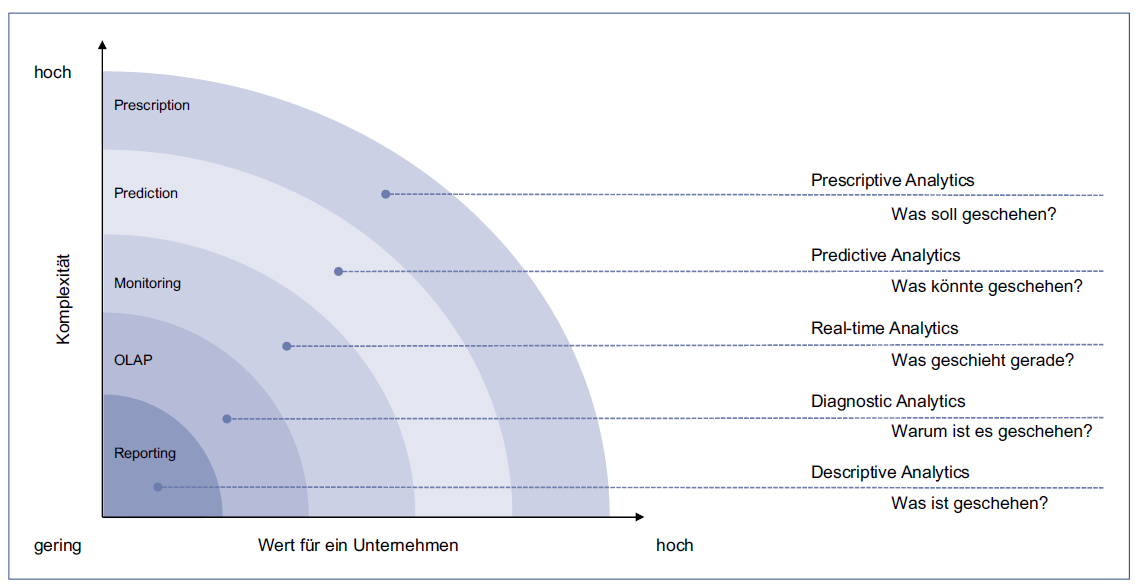
\includegraphics[width=16cm]{Abbildungen/Analysis.png}
\caption{Analysis Questions \cite{2}}\label{visina8}
\end{figure*}


As you can see in Figure 2, the questions which can be asked and answered  each provide a different solution of the Business-Analytic-System. Within the scope of the application areas of business analytics, only descriptive analytics, diagnostic analytics and real-time analytics are used. The descriptive analytics follow the classic concept of reporting, which analyses the situation in terms of what has happened and when did it happen. Diagnostic analytics follows the investigative approach. The main question here is why this situation could have arisen. The last shown possibility of the application field of analysis corresponds to the principle of real-time analytics. These are based on monitoring systems which are currently in running in a system. 

\subsubsection{Application Area - Forecast}
Forecasting is a business analytics tool that uses stochastic models, machine learning and data mining approaches to make efficient forecasts with good results (cf. Mehanna et al. \cite{2}). There is an additional distinction to the so-called digital forecasts as well. The digital forecasts can be used in such a way that at the end, for example, by combining several of these digital forecasts, to forecast the so-called EBITDA (earnings before interest, taxes, depreciation and amortization). In this example, the following forecasts have been combined. First, the "sales forecasts based on unstructured data on trends". In addition, a forecast for "fully automated pricing". This is followed by an "early detection of changes in raw material prices" and last but not least, one for "optimization of warehousing" (cf. Mehanna et al. \cite{2}). The result is a continuously learning sales forecast, which could be used for the application area of the optimization.

\subsubsection{Application Area - Optimization}
With the help of forecasts or digital forecasts, you receive information about the future development of the areas on which the forecasting was applied. This alone is not enough to allow the company to operate more economically though. Another important factor is optimization. The optimization procedure follows the forecasting procedure. A very good example of optimization is to optimize the inventory in the retail trade. There the system is automatically adjusted so that, when a customer orders an article, it is automatically offset against the stock quantity of the article in the warehouse. As soon as a predefined minimum is reached, this article is going to be reordered automatically by the system (cf. Mehanna et al. \cite{2}). The model explained in this example reduces both the cost of the company's stock and the cost of ordering new goods. However, not the actual cost of the goods. \textit{'Models for identifying new cause-effect relationships can be continuously developed and thus generate new insights into bottlenecks or inefficiencies. On the other hand, automated analyses shorten reaction times, enable "high-frequency decisions" and lead continuously to ad-hoc implementation of optimization measures.'}\cite{2}. The focus of the optimization process should be on the continuous optimization of the overall system.

\subsubsection{Application Area - Simulation}
The simulation process describes the simulation of a company and possible future developments. \textit{'Various scenarios for possible corporate development are already being simulated today, for example in the context of corporate planning. At present, however, most of these simulations are characterized by high manual effort and personnel commitment. In addition, the short-term response to changes in the scenarios is very limited. As a result, simulations for corporate management are often reduced to a minimum and thus cannot unfold their added value. Potentially highly relevant control information will be lost.'} \cite{2}. What Mehanna et al. are talking about, is that the user of simulations often do not offer enough meaning, attention and resources of any kind. If they were properly designed and fed with all relevant data, they could be used to support operational decisions. For this type of simulation, there are driver-based models, such as the revenue control model. The aim of the revenue management model is to ensure, that the available resources of all kinds generate the highest revenue. In the best case, the business analytics forecast is the basis of this model. All relevant data, such as capacity, prices, load, operating time, etc., are loaded into the revenue control model. The results of this simulation are, for example, optimized prices at certain selling points (cf. Mehanna et al. \cite{2}). It should be noted here that the simulation is a kind of learning algorithm and that in the best case this should also be fed with actual values so that these are taken into account in the forthcoming simulations. 


\subsubsection{Application Area - Radar}
The radar method is the continuous observation and analysis of the market segment in which the company operates. This is where the term competitive intelligence comes into play. Competitive intelligence combines processes and technologies for clarifying the market and its associated components, such as patents, customers, suppliers, competitors, etc. (cf. Mehanna et al. \cite{2}). The basis for useful data that can be fed into the radar are social media channels and basically, everything that can be summerized as "open data". Open data includes public sites as well as forums and websites of different companies, which are in the same market segment. This information is analysed using semantic analyses. These include methods such as natural language processing or text mining. Furthermore, all relevant information or findings should be obtained in the radar procedure. These can help a company to make its own brand more competitive, since it can also evaluate external characteristics, such as the perception of its own brand by a customer. Thanks to radar, more resources can and will be invested in innovations, which explains the current growth in product diversity.



\subsection{What has to be considered with Business Analytics?}
So far, this paper has only reported positively from Business Analytics. Then how come not every company works with business analytics? One of the reasons is that the investment in the technology itself is relatively expensive and does not solve all problems. It is also important that the users must be able to limit the problems and then run their analyses on them. Only those who provide the right data for the right analysis in advance will possibly arrive at useful results. Furthermore, it is not only relevant which data is made available for analysis, but also with which algorithm it is processed. Additionally, the type of visualization of the results is added. As long as these are not presented in a meaningful way, the most effective algorithms and the best data are useless. Last but not least, it is always the final interpretation of the competent authority. As can be concluded from this, there are also a considerable amount of risks in business analytics. So how should business analytics be used? Carsten Felden explained it in his blog as follows: \textit{'First of all, when introducing business analytics, the added value for the company must be determined, since the benefits acquired must justify the effort. Another fact is the underlying project-oriented and process-oriented approach. The project-oriented characteristic results from the fact that it is in the nature of data mining approaches, for example, not to be a control loop. New data must be compiled for the respective value-creating tasks, goal-oriented analysis options for the underlying data must be evaluated and executed in order to be able to use the results in daily business operations.'} \cite{4}. As the text by Carsten Felden shows, it should first be considered whether the area of application of the company reflects any benefit for business analytics or not. Then it is important that the system is or can be permanently supplied with meaningful information. If these points do not speak in favour, the company should not opt for a solution approach based on business analytics.

\subsection{Business Analytics - Analysis algorithms}
Since business analytics is more an approach than a concrete solution, there are various analysis tools. Here are some of the most popular:

\begin{itemize}
\item A/B tests
\item Statistical or quantitative analysis
\item Text Mining
\item Data Mining
\item Predictive Analytics
\end{itemize}

While A/B tests, statistical or quantitative analysis and data mining are already quite precise approaches to plan a company's future course, are predictive analytics a subfield of business analytics. Lets first talk about data mining.

\section{Knowledge Discovery in Databases(KDD) }


\subsection{KDD - Process}
Basically, data mining is a partial step of data analysis and knowledge discovery in databases processes. \textit{The aim of the KDD is the recognition of so far unknown technical connections from existing, mostly large data sets. In contrast to data mining, KDD also includes the preparation of the data and the evaluation of the results as an overall process.'} \cite{3}.

\begin{figure*}
\centering
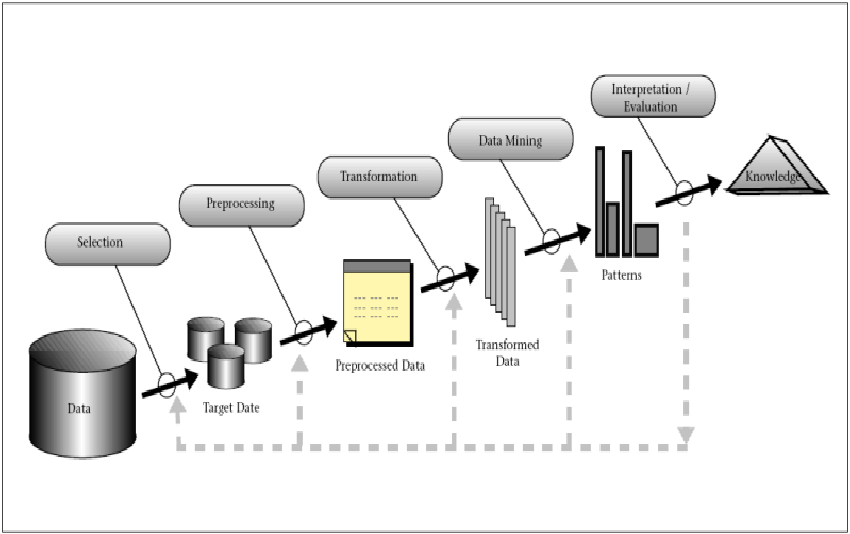
\includegraphics[width=16cm]{Abbildungen/KDD.png}
\caption{KDD Process \cite{11} }\label{visina8}
\end{figure*}

As Figure 3 shows, the KDD process consists of several steps. The first step, the selection step, consists of first picking out data that could have a meaning for the analysis which is going to be carried out. These are then preprocessed, where erroneous data is removed or corrected. What follows is the process of data reduction, in which the data is reduced to its content which is going to be processed. After that the step of data mining, where the actual data analysis is performed, is happening. The result of the data mining is pushed into different, previousl selected patterns which are finally ready to be interpreted by the user.


\subsection{KDD - Data Mining Application Procedures}
The procedures in which a data mining application works differ from company to company and even there from situation to situation depending on the wanted outcome. The typical procedures are essentially divided into the following:

\begin{itemize}
\item Anomaly analysis
\item Cluster analyses
\item Classification
\item Association analyses
\item Regression analysis
\end{itemize}

\subsubsection{Anomaly analysis}
Anomaly analysis is a type of analysis in which an average is formed and any data set that differs too much from this average is marked as suspicious. It is usual that data records marked as suspicious are manually checked for correctness by a user {cf. Alpar, Paul et al. \cite{14}}.

\subsubsection{Cluster analyses}
In so-called cluster analyses, the data sets are analysed in certain concentrations within a data room. If a data set does not fit into a cluster, it is marked as suspicious, depending on the type of procedure, as in anomaly analysis. Here too, data records marked as suspicious are checked for correctness by a user {cf. Alpar, Paul et al. \cite{14}}.

\subsubsection{Classification}
Similar to cluster analyses, the data records are analysed and mapped into a data room when classifying data. However, unlike cluster analysis, these rooms are predefined before the analysis procedure {cf. Alpar, Paul et al. \cite{14}}.  

\subsubsection{Association analyses}
The association analyses search for normality or rule cases in the data sets. These results could, for example, indicate what kind of objects are related to each other in some way {cf. Alpar, Paul et al. \cite{14}}.

\subsubsection{Regression analysis}
The association analyses search for normality or rule cases in the data sets. These results could, for example, indicate what kind of objects are related to each other in some way {cf. Alpar, Paul et al. \cite{14}}.

\subsection{KDD - Data Mining specializations}
A frequently used algorithm for big data analysis is data mining. However, since there is an unmanageable amount of possibilities to analyse other data types, the data mining algorithm can be divided into many special modifications. Those specializations start where the normal data mining algorithm reaches its limits. Since there is a different data mining algorithm for almost each  data type, only a few are mentioned here. On the one hand, there is text mining, which is an analysis procedure that analyses textual data. With data mining, text mining is probably one of the best-known analysis methods. An example application is represented in the so-called plagiarism determination. Another specialized modification is web mining. Web mining is based on the algorithms of cluster analysis and association analysis. This is used by some search engines, for example. 


\section{Predictive Analytics}
\subsection{Predictive Analytics - Methodical aspects}
Since predictive analytics focuses on predicting future events, there are also a few methodological requirements for the process. On the one hand, it depends on the origin of the used information. It is important that only trustworthy information from the immediate environment or data/information which was collected by oneself is used. It is also neccesary that the user who evaluates the results also gets to see the values of the analysis in addition to the results. On the other hand, it is important that the methods used to carry out the analysis, take into account the market environment or the industry. One of the methodological peculiarities is that the system is modeled from the user's point of view, predefined connections and restrictions so that the system can work effectively for the respective application (cf. Baars \cite{1}).

\subsection{Predictive Analytics - Architectural Aspects}
With a predictive analytics system, it is recommended to use several systems that are responsible for the analysis. For these purposes, it would make sense to operate a system separate from the production system in the form of a sandbox. Furthermore, it requires high-quality data to generate models. This data, relevant for analysis and model generation, should be both internal and external in nature. For the sandbox system, it is also recommended to have a number of tools available, for example data mining tools as well as data manipulation and data integration tools (cf. Baars \cite{1}). The combination of all these technical aspects serves to be able to observe an analysis process and to transfer the resulting information and experience into the production system. 

\section{Conclusion}
\subsubsection{Application Area - Resume}

Business analytics and the therin contained  knowledge discovery in databases and predictive analytics are approaches that could appeal to every IT industry, since the digitization of corporate management with big data and business analytics could trigger a paradigm shift (cf. Mehanna et al. [2]). It makes no difference whether it is used in a normal retail trade or in banks. Each of these sectors could benefit tremendously from a correctly implemented business analytics system. Then why hasn't it been implemented everywhere? Costs are a big argument against business analytics. The costs involved in setting up a complete business analytics system with all components are immensely high. Furthermore, a certain amount of time must first pass under observation before the system can belong to the production system. The last and most important point, is the controlling personnel. In the end, it does not matter how the system was implemented, if the staff evaluates or interprets the results of the analysis "incorrectly", it may be that a company takes a wrong course and as result will the profitability of the company  suffer. Another problem is that the data-driven control is far from being perfected. However, there are also a lot of positive examples of the use of business analytics and more precisely the use of predictive analytics. For example, the global player IBM has been using predictive analytics for years and even offers services and tools for company optimization purposes. In my opinion should the whole subject be treated with caution and the decision of using predictive analytics should be considered carefully and should be treatened with a lot of care and attention, but the whole topic is definetily worth observing. Who knows, it might be possible to create some kind of template for implementing predictive analytic systems in a company.
\newpage

\begin{thebibliography}{99}
\bibitem{1}
	Dr. Henning Baars 2016: Predictive Analytics in der IT-basierten Entscheidungsunterstützung – methodische, architektonische und 			organisatorische Konsequenzen

\bibitem{2}
	Mehenna et al. 2016: Business Analytics im Controlling – Fünf Anwendungsfelder

\bibitem{3}
	Martin Ester, Jörg Sander 2000: Knowledge Discovery in Databases: Techniken und Anwendungen. 
\bibitem{4}
http://www.enzyklopaedie-der-wirtschaftsinformatik.de/lexikon/daten-wissen/Business-Intelligence/Analytische-Informationssysteme--Methoden-der-/Business-Analytics
Called on 14.06.2018 at 10:15 AM CEST

\bibitem{5}
 https://www.gartner.com/it-glossary/business-intelligence-bi/ Called on 16.06.2018 at 3:28 PM CEST

\bibitem{6}
https://abas-erp.com/de/news/business-analytics-vs-business-intelligence-wo-liegen-die-unterschiede Called on 16.06.2018 at 6:13 PM CEST

\bibitem{7}
https://barc.de/news/business-intelligence-fur-alle-bleibt-zukunftsmusik
Called on 17.06.2018 at 09:30 AM CEST

\bibitem{8}
https://www.computerwoche.de/a/was-ist-was-bei-predictive-analytics
Called on 19.06.2018 at 08:03 AM CEST

\bibitem{9}
https://www.horvath-partners.com/fileadmin/user-upload/E-Business-Intelligence-Magazine-Mehanna-Digital-Forecasts.pdf
Called on 19.06.2018 at 12:03 PM CEST

\bibitem{10}
http://www.enzyklopaedie-der-wirtschaftsinformatik.de/lexikon/daten-wissen/Business-Intelligence/Members/felden/BAProzess.png
called on 14.06.2018 at 3:35 PM CEST

\bibitem{11}
https://www.researchgate.net/profile/Sohaib-Latif/publication/259757435/figure/fig2/AS:297124118974477@1447851318372/Overview-of-the-steps-consulting-the-KDD-process.png 
called on 19.06.2018 at 11:53 PM CEST

\bibitem{12}
https://www.industry-press.com/business-analytics-tools/
called on 19.06.2018 at 1:37 PM CEST

\bibitem{13}
https://www.linkfish.eu/wie-eine-bi-strategie-formuliert-und-implementiert-werden-kann/
called on 20.06.2018 at 4:45 PM CEST

\bibitem{14}
Alpar, Paul und Niederreichholz, Joachim (2000), Data Mining im praktischen Einsatz: Verfahren und Anwendungsfälle für Marketing, Vertrieb, Controlling und Kundenunterstützung

\end{thebibliography}
\end{document}
